The purpose of this case is to test the loss ratio sampling when the Beta vulnerability model has nonzero coefficients of variation of the loss ratios. Table~\ref{tab:vf-ln-tax1-nzcov} shows the mean loss ratios and corresponding coefficients of variation in the vulnerability model used in this test case.

Apart from the nonzero coefficients of variation in the vulnerability model, this case is similar to Case~1e. The only difference enters during the loss ratio sampling stage, where the Beta distribution no longer devolves into the degenerate distribution.

% The loss curve calculated using the implementation of the calculator in Julia is compared with that produced by OpenQuake in Figure~\ref{fig:lc-ebr-1f}.

% \begin{figure}[htbp]
% \centering
% 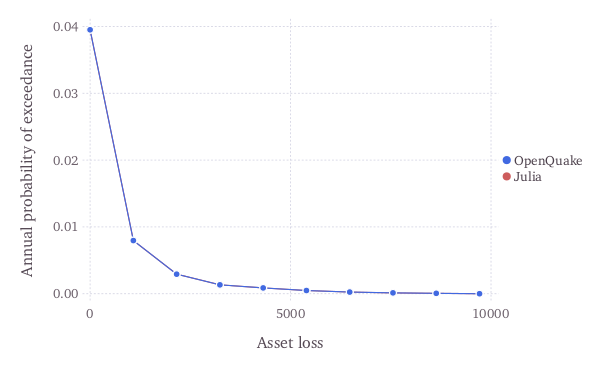
\includegraphics[width=12cm]{qareport/figures/fig-lc-ebr-1f}
% \caption{Loss curve comparison for event based risk test case 1f}
% \label{fig:lc-ebr-1f}
% \end{figure}

The area under the annual loss exceedance curve gives the average annual loss.